% Options for packages loaded elsewhere
\PassOptionsToPackage{unicode}{hyperref}
\PassOptionsToPackage{hyphens}{url}
\PassOptionsToPackage{dvipsnames,svgnames*,x11names*}{xcolor}
%
\documentclass[
  10pt,
]{article}
\usepackage{amsmath,amssymb}
\usepackage{lmodern}
\usepackage{ifxetex,ifluatex}
\ifnum 0\ifxetex 1\fi\ifluatex 1\fi=0 % if pdftex
  \usepackage[T1]{fontenc}
  \usepackage[utf8]{inputenc}
  \usepackage{textcomp} % provide euro and other symbols
\else % if luatex or xetex
  \usepackage{unicode-math}
  \defaultfontfeatures{Scale=MatchLowercase}
  \defaultfontfeatures[\rmfamily]{Ligatures=TeX,Scale=1}
\fi
% Use upquote if available, for straight quotes in verbatim environments
\IfFileExists{upquote.sty}{\usepackage{upquote}}{}
\IfFileExists{microtype.sty}{% use microtype if available
  \usepackage[]{microtype}
  \UseMicrotypeSet[protrusion]{basicmath} % disable protrusion for tt fonts
}{}
\makeatletter
\@ifundefined{KOMAClassName}{% if non-KOMA class
  \IfFileExists{parskip.sty}{%
    \usepackage{parskip}
  }{% else
    \setlength{\parindent}{0pt}
    \setlength{\parskip}{6pt plus 2pt minus 1pt}}
}{% if KOMA class
  \KOMAoptions{parskip=half}}
\makeatother
\usepackage{xcolor}
\IfFileExists{xurl.sty}{\usepackage{xurl}}{} % add URL line breaks if available
\IfFileExists{bookmark.sty}{\usepackage{bookmark}}{\usepackage{hyperref}}
\hypersetup{
  pdftitle={Geburtsdataset analysis},
  pdfauthor={Zehui Bai},
  colorlinks=true,
  linkcolor=Maroon,
  filecolor=Maroon,
  citecolor=Blue,
  urlcolor=Blue,
  pdfcreator={LaTeX via pandoc}}
\urlstyle{same} % disable monospaced font for URLs
\usepackage[margin=1in]{geometry}
\usepackage{longtable,booktabs,array}
\usepackage{calc} % for calculating minipage widths
% Correct order of tables after \paragraph or \subparagraph
\usepackage{etoolbox}
\makeatletter
\patchcmd\longtable{\par}{\if@noskipsec\mbox{}\fi\par}{}{}
\makeatother
% Allow footnotes in longtable head/foot
\IfFileExists{footnotehyper.sty}{\usepackage{footnotehyper}}{\usepackage{footnote}}
\makesavenoteenv{longtable}
\usepackage{graphicx}
\makeatletter
\def\maxwidth{\ifdim\Gin@nat@width>\linewidth\linewidth\else\Gin@nat@width\fi}
\def\maxheight{\ifdim\Gin@nat@height>\textheight\textheight\else\Gin@nat@height\fi}
\makeatother
% Scale images if necessary, so that they will not overflow the page
% margins by default, and it is still possible to overwrite the defaults
% using explicit options in \includegraphics[width, height, ...]{}
\setkeys{Gin}{width=\maxwidth,height=\maxheight,keepaspectratio}
% Set default figure placement to htbp
\makeatletter
\def\fps@figure{htbp}
\makeatother
\setlength{\emergencystretch}{3em} % prevent overfull lines
\providecommand{\tightlist}{%
  \setlength{\itemsep}{0pt}\setlength{\parskip}{0pt}}
\setcounter{secnumdepth}{-\maxdimen} % remove section numbering
\ifluatex
  \usepackage{selnolig}  % disable illegal ligatures
\fi

\title{Geburtsdataset analysis}
\author{Zehui Bai}
\date{Stand: 2021-11-08 19:56 Uhr}

\begin{document}
\maketitle

{
\hypersetup{linkcolor=}
\setcounter{tocdepth}{2}
\tableofcontents
}
\hypertarget{descriptive-statistics-of-variables}{%
\subsection{Descriptive statistics of
variables}\label{descriptive-statistics-of-variables}}

\hypertarget{descriptive-statistics-for-gewichtszunahme-mutter-alter-mutter-bmi}{%
\subsubsection{Descriptive statistics for Gewichtszunahme, Mutter Alter,
Mutter
BMI}\label{descriptive-statistics-for-gewichtszunahme-mutter-alter-mutter-bmi}}

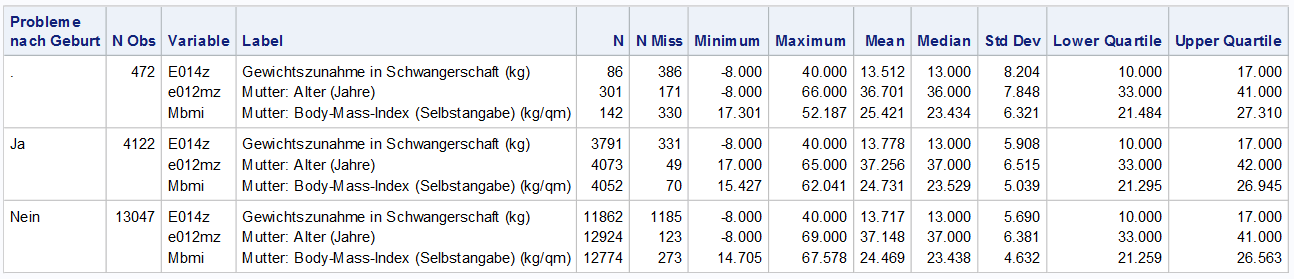
\includegraphics[width=17.97in]{./Yimeng_Plots/M7_0a}

\hypertarget{descriptive-statistics-for-geschlecht}{%
\subsubsection{Descriptive statistics for
Geschlecht}\label{descriptive-statistics-for-geschlecht}}

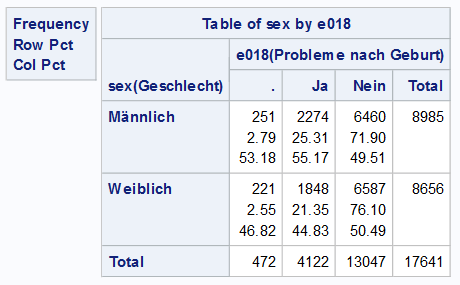
\includegraphics[width=6.39in]{./Yimeng_Plots/M7_0b}

\hypertarget{descriptive-statistics-for-mutter-schulabschluss}{%
\subsubsection{Descriptive statistics for Mutter:
Schulabschluss}\label{descriptive-statistics-for-mutter-schulabschluss}}

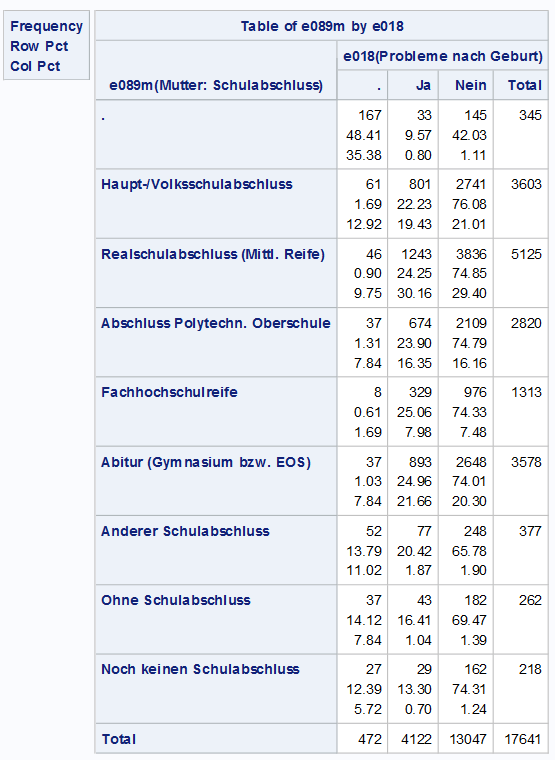
\includegraphics[width=7.71in]{./Yimeng_Plots/M7_0c}

\hypertarget{descriptive-statistics-for-monatl.-haushaltsnettoeinkommen}{%
\subsubsection{Descriptive statistics for Monatl.
Haushaltsnettoeinkommen}\label{descriptive-statistics-for-monatl.-haushaltsnettoeinkommen}}

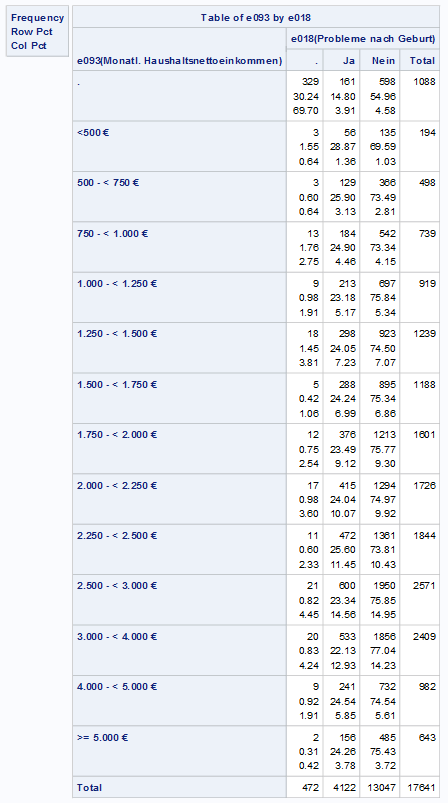
\includegraphics[width=6.22in]{./Yimeng_Plots/M7_0d}

\hypertarget{descriptive-statistics-for-ostwest-geografisch}{%
\subsubsection{Descriptive statistics for Ost/West
geografisch}\label{descriptive-statistics-for-ostwest-geografisch}}

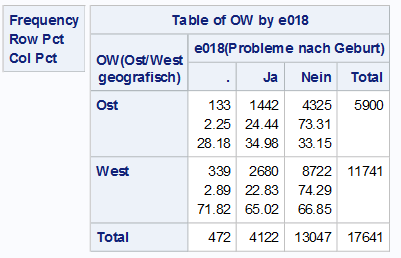
\includegraphics[width=5.57in]{./Yimeng_Plots/M7_0e}

\hypertarget{nach-geburt}{%
\subsubsection{Nach Geburt}\label{nach-geburt}}

\begin{longtable}[]{@{}lll@{}}
\toprule
& N & \% \\
\midrule
\endhead
Probleme Nach Geburt & 4122 & \\
Atmungsschwierigkeiten, Anpassungsstörungen & 645 & 15.65 \\
Infektion & 450 & 10.92 \\
Gelbsucht & 2112 & 51.24 \\
Untergewicht, Frühgeburt & 763 & 18.51 \\
Sonstige & 947 & 22.97 \\
Kinderklinik & 1616 & 39.20 \\
\bottomrule
\end{longtable}

\hypertarget{full-model}{%
\subsection{Full model}\label{full-model}}

\begin{itemize}
\tightlist
\item
  并未发现Gewichtszunahme in Schwangerschaft (kg)是Probleme nach
  Geburt的显著影响因素
\item
  但是发现了Mutter: Body-Mass-Index (kg/qm)对Probleme nach
  Geburt影响很大
\item
  显然Ost/West geografisch对Probleme nach Geburt无影响,从模型中提出
\end{itemize}

下表是全模型的分析结果

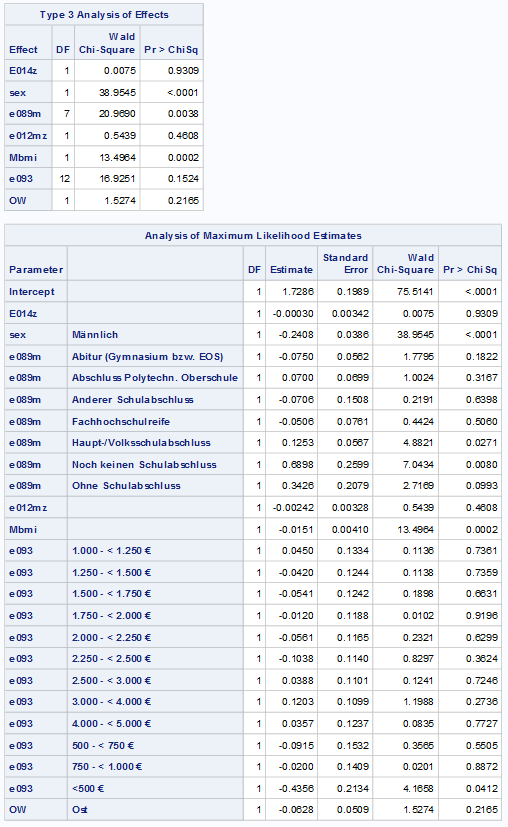
\includegraphics[width=7.06in]{./Yimeng_Plots/M7_1}

\hypertarget{new-model}{%
\subsection{New Model}\label{new-model}}

结果和简单的解释如下

\begin{itemize}
\tightlist
\item
  显然Sex具有显著性,女孩得病的风险更高
\item
  母亲受教育水平越高,孩子得病风险相对于没有毕业的人的孩子越小
\item
  家庭收入影响不显著,但有意思的是特别高收入人群的孩子相反更容易生病
  (\textgreater= 5.000 € vs \textless500 €,e093 4.000 - \textless{}
  5.000 € vs \textless500
  €)但是low置信区间接近1,因此不能说明有普遍效应
\item
  母亲的bmi对孩子的健康有所影响,bmi越高,生病可能性越大
\end{itemize}

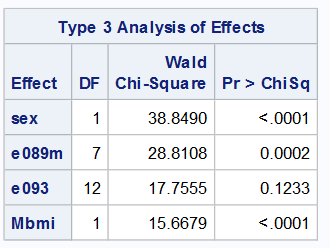
\includegraphics[width=4.58in]{./Yimeng_Plots/M7_2}
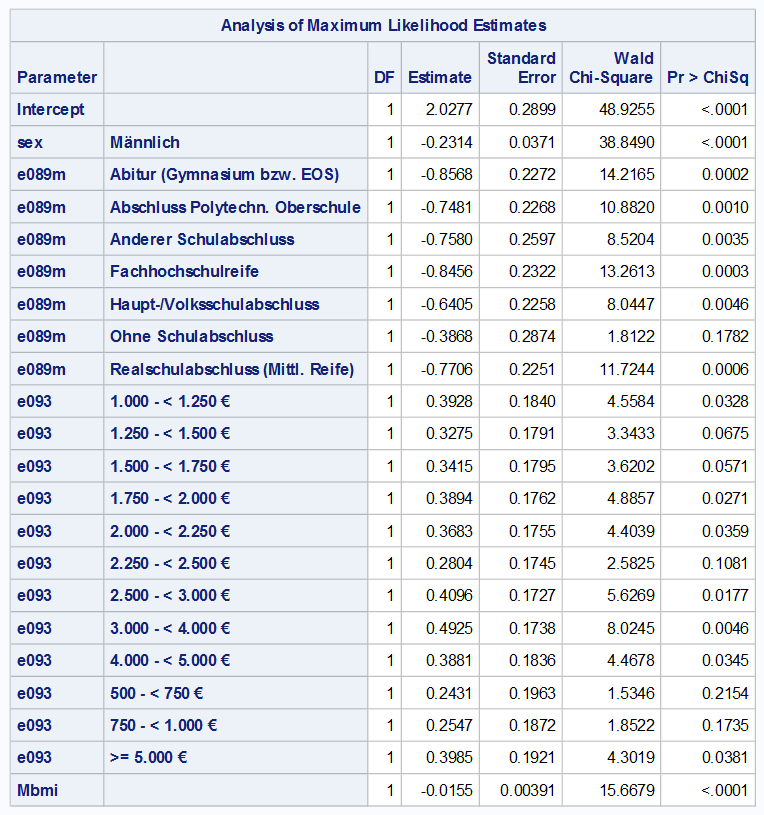
\includegraphics[width=10.61in]{./Yimeng_Plots/M7_4}
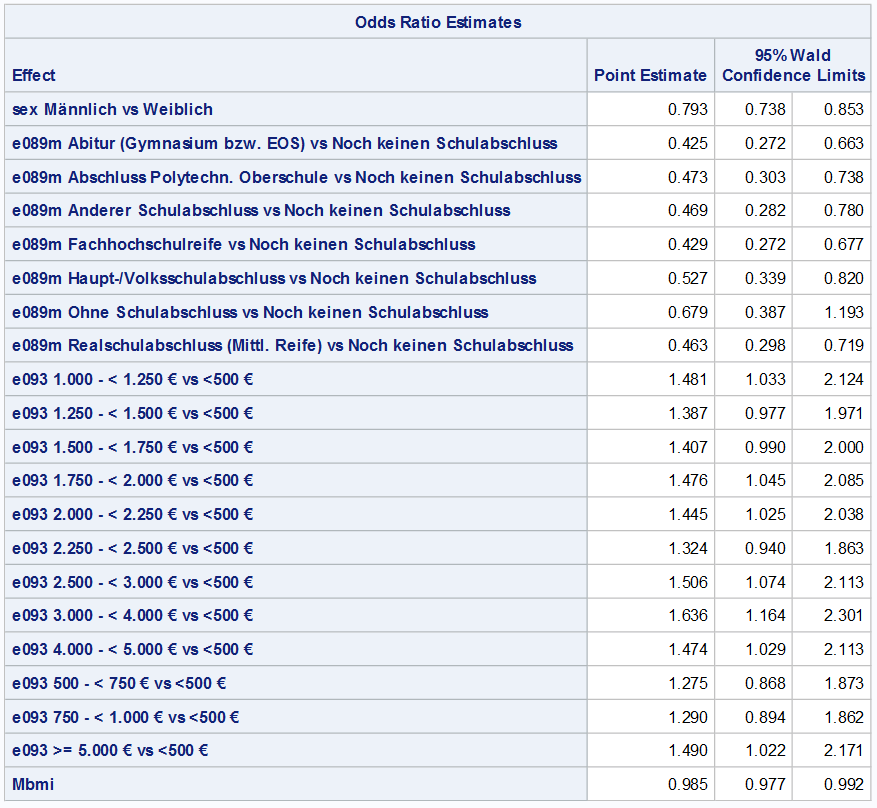
\includegraphics[width=12.18in]{./Yimeng_Plots/M7_5}
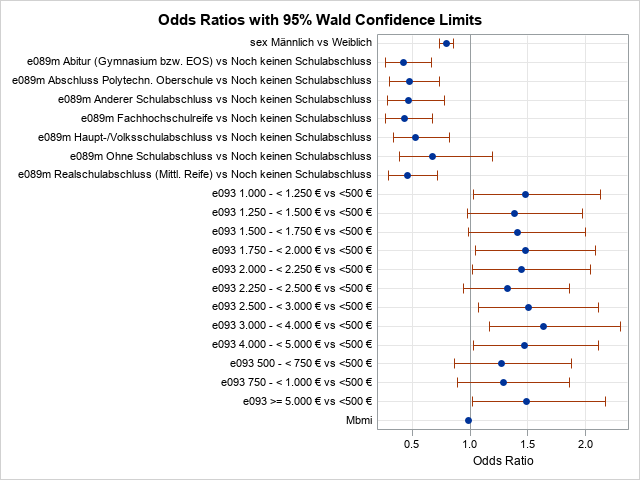
\includegraphics[width=8.89in]{./Yimeng_Plots/M7_3}

\end{document}
